\chapter{Sprint 4 : Planification visuelle et notifications}

\section*{Introduction}
Le quatrième sprint apporte les outils de visualisation décisionnelle : diagramme de
Gantt interactif avec calcul automatique du chemin critique (algorithme CPM),
calendrier mensuel des tâches, système de notifications temps réel via WebSocket
(Laravel Reverb), et tableaux de bord différenciés selon le profil de l'utilisateur.

% ============================================================
\section{Sprint Backlog}

\begin{table}[H]
  \centering
  \caption{Sprint Backlog — Sprint 4}
  \label{tab:backlog_s4}
  \begin{tabularx}{\textwidth}{C{1.2cm}L{5.5cm}L{2cm}C{2cm}C{1.5cm}}
    \toprule
    \thead{ID} & \thead{User Story} & \thead{Acteur} & \thead{Priorité} & \thead{Points} \\
    \midrule
    \rowcolor{lightgray}
    US-17 & Visualiser le Gantt avec chemin critique     & Member & Must   & 13 \\
    US-18 & Consulter le calendrier mensuel              & Member & Should &  5 \\
    \rowcolor{lightgray}
    US-19 & Recevoir des notifications temps réel        & Tous   & Must   &  8 \\
    US-20 & Configurer ses préférences de notification   & Tous   & Should &  3 \\
    \rowcolor{lightgray}
    US-21 & Accéder à un dashboard personnel             & Member & Should &  8 \\
    US-22 & Accéder au dashboard administrateur          & Admin  & Should &  5 \\
    \rowcolor{lightgray}
    US-27 & Consulter le rapport d'avancement (client)   & Client & Should &  5 \\
    US-28 & Utiliser la recherche globale                & Tous   & Should &  5 \\
    \midrule
    \multicolumn{4}{r}{\textbf{Total :}} & \textbf{52} \\
    \bottomrule
  \end{tabularx}
\end{table}

% ============================================================
\section{Conception}

\subsection{Diagramme de cas d'utilisation}

\begin{figure}[H]
  \centering
  \IfFileExists{figures/sprint4_use_case.png}{%
    \includegraphics[width=0.88\textwidth]{figures/sprint4_use_case.png}%
  }{%
    \fbox{\parbox{0.88\textwidth}{\centering\vspace{1.8cm}
      \textbf{[IMAGE A INSÉRER]}\\[0.4em]
      \texttt{figures/sprint4\_use\_case.png}\\[0.3em]
      \textit{Cas d'utilisation : Admin, Member, Client — Gantt, calendrier, notifications, dashboards}
    \vspace{1.8cm}}}%
  }
  \caption{Diagramme de cas d'utilisation — Sprint 4}
  \label{fig:uc_s4}
\end{figure}

\subsection{Diagramme de séquence — Détection de retard et notification}

\begin{figure}[H]
  \centering
  \IfFileExists{figures/sprint4_sequence_notif.png}{%
    \includegraphics[width=0.90\textwidth]{figures/sprint4_sequence_notif.png}%
  }{%
    \fbox{\parbox{0.90\textwidth}{\centering\vspace{1.8cm}
      \textbf{[IMAGE A INSÉRER]}\\[0.4em]
      \texttt{figures/sprint4\_sequence\_notif.png}\\[0.3em]
      \textit{Séquence : Scheduler horaire → détection retard → NotificationService → Reverb WebSocket}
    \vspace{1.8cm}}}%
  }
  \caption{Diagramme de séquence — Notification de retard (scheduler horaire)}
  \label{fig:seq_notif}
\end{figure}

Le scheduler Laravel s'exécute toutes les heures : il sélectionne les tâches dont la
\texttt{due\_date} est dépassée et dont le \texttt{workflow\_status} n'est pas
\texttt{done}. Pour chaque tâche concernée, \texttt{NotificationService::notifyDelay()}
persiste une notification en base et diffuse l'événement \texttt{TaskDelayed}
sur le canal privé \texttt{private-user.\{id\}}. Côté React, le badge de la cloche
s'incrémente et un toast apparaît.

\subsection{Diagramme de classes}

\begin{figure}[H]
  \centering
  \IfFileExists{figures/sprint4_class.png}{%
    \includegraphics[width=0.85\textwidth]{figures/sprint4_class.png}%
  }{%
    \fbox{\parbox{0.85\textwidth}{\centering\vspace{1.8cm}
      \textbf{[IMAGE A INSÉRER]}\\[0.4em]
      \texttt{figures/sprint4\_class.png}\\[0.3em]
      \textit{Classes : Notification, ActivityLog, CriticalPathService, AdminDashboardService}
    \vspace{1.8cm}}}%
  }
  \caption{Diagramme de classes — Sprint 4}
  \label{fig:class_s4}
\end{figure}

% ============================================================
\section{Réalisation}

\subsection{Diagramme de Gantt}

\begin{figure}[H]
  \centering
  \IfFileExists{figures/sprint4_19_gantt.png}{%
    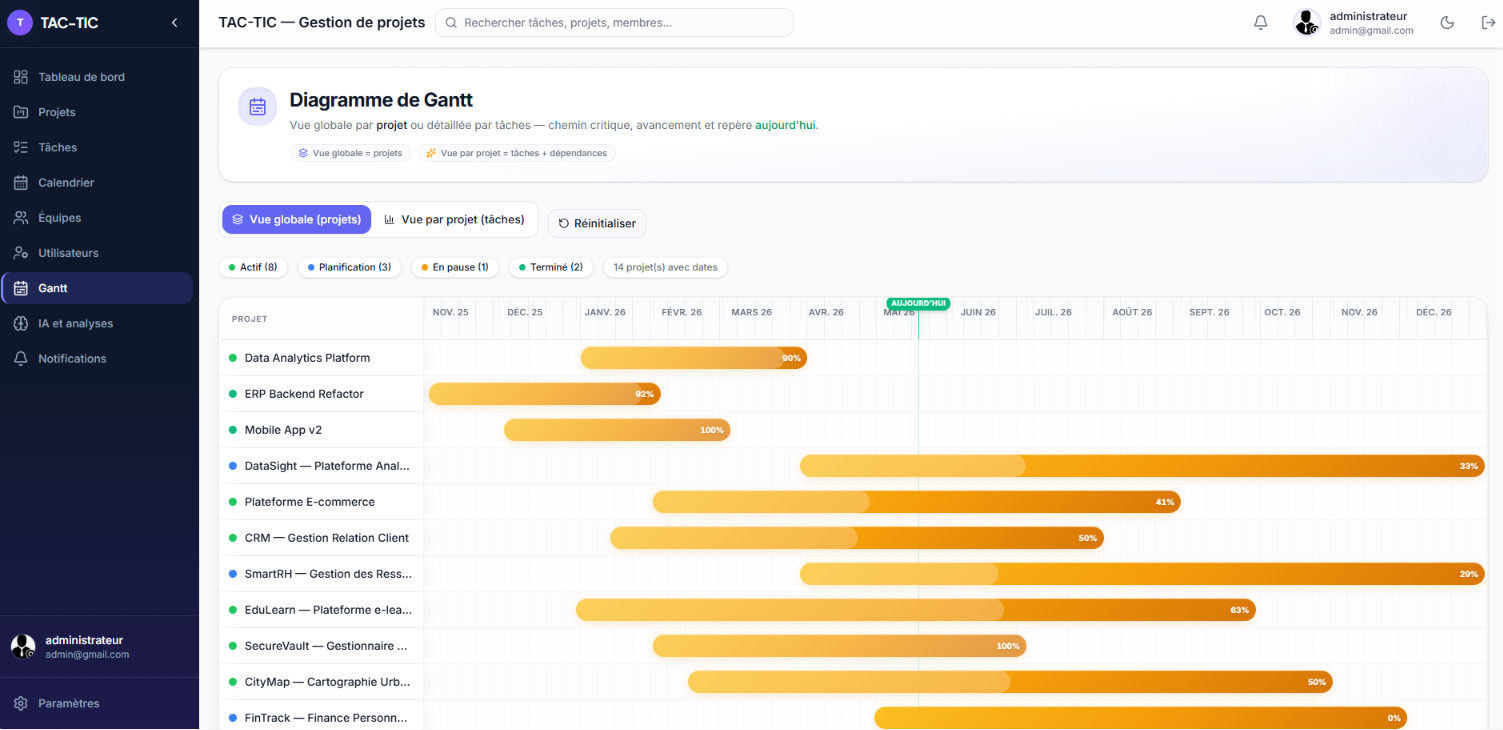
\includegraphics[width=0.92\textwidth]{figures/sprint4_19_gantt.png}%
  }{%
    \fbox{\parbox{0.92\textwidth}{\centering\vspace{2cm}
      \textbf{[IMAGE A INSÉRER]}\\[0.4em]
      \texttt{figures/sprint4\_19\_gantt.png}\\[0.3em]
      \textit{Gantt : 12 projets janv.--déc. 2026, repère AUJOURD'HUI, couleurs par priorité,
      chemin critique en rouge dans la vue projet}
    \vspace{2cm}}}%
  }
  \caption{Diagramme de Gantt interactif — Vue globale multi-projets}
  \label{fig:ui_gantt}
\end{figure}

Le Gantt est rendu entièrement en SVG côté client. Chaque barre représente une tâche ;
sa couleur encode la priorité. Le repère vertical « AUJOURD'HUI » est calculé
dynamiquement. Dans la vue projet, les tâches du chemin critique (float = 0) sont
affichées en rouge. Un survol de barre affiche une infobulle avec titre, dates et
progression.

\subsection{Calendrier mensuel}

\begin{figure}[H]
  \centering
  \IfFileExists{figures/sprint4_20_calendar.png}{%
    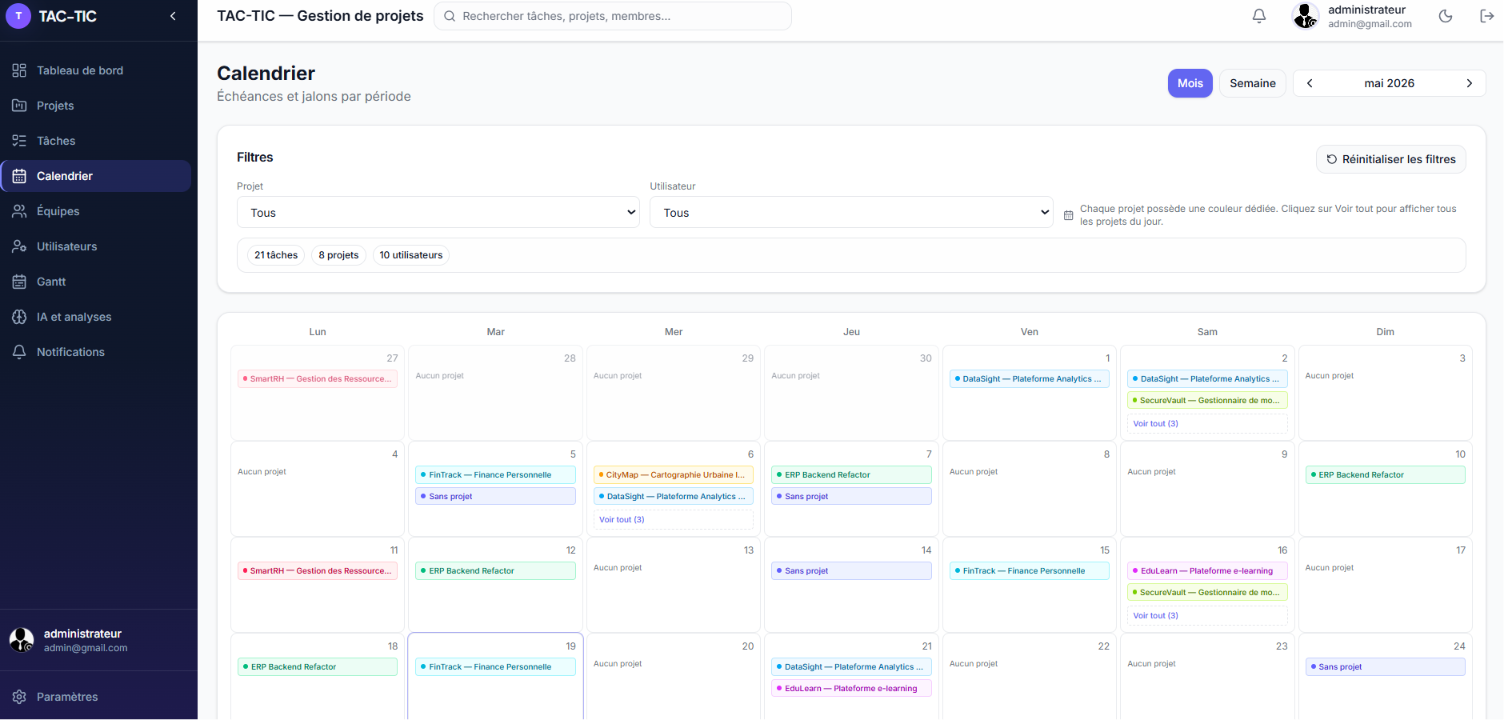
\includegraphics[width=0.88\textwidth]{figures/sprint4_20_calendar.png}%
  }{%
    \fbox{\parbox{0.88\textwidth}{\centering\vspace{2cm}
      \textbf{[IMAGE A INSÉRER]}\\[0.4em]
      \texttt{figures/sprint4\_20\_calendar.png}\\[0.3em]
      \textit{Calendrier Mai 2026, filtres projet/utilisateur, événements colorés par priorité}
    \vspace{2cm}}}%
  }
  \caption{Calendrier mensuel — Mai 2026}
  \label{fig:ui_calendar}
\end{figure}

\subsection{Centre de notifications}

\begin{figure}[H]
  \centering
  \IfFileExists{figures/sprint4_21_notifications.png}{%
    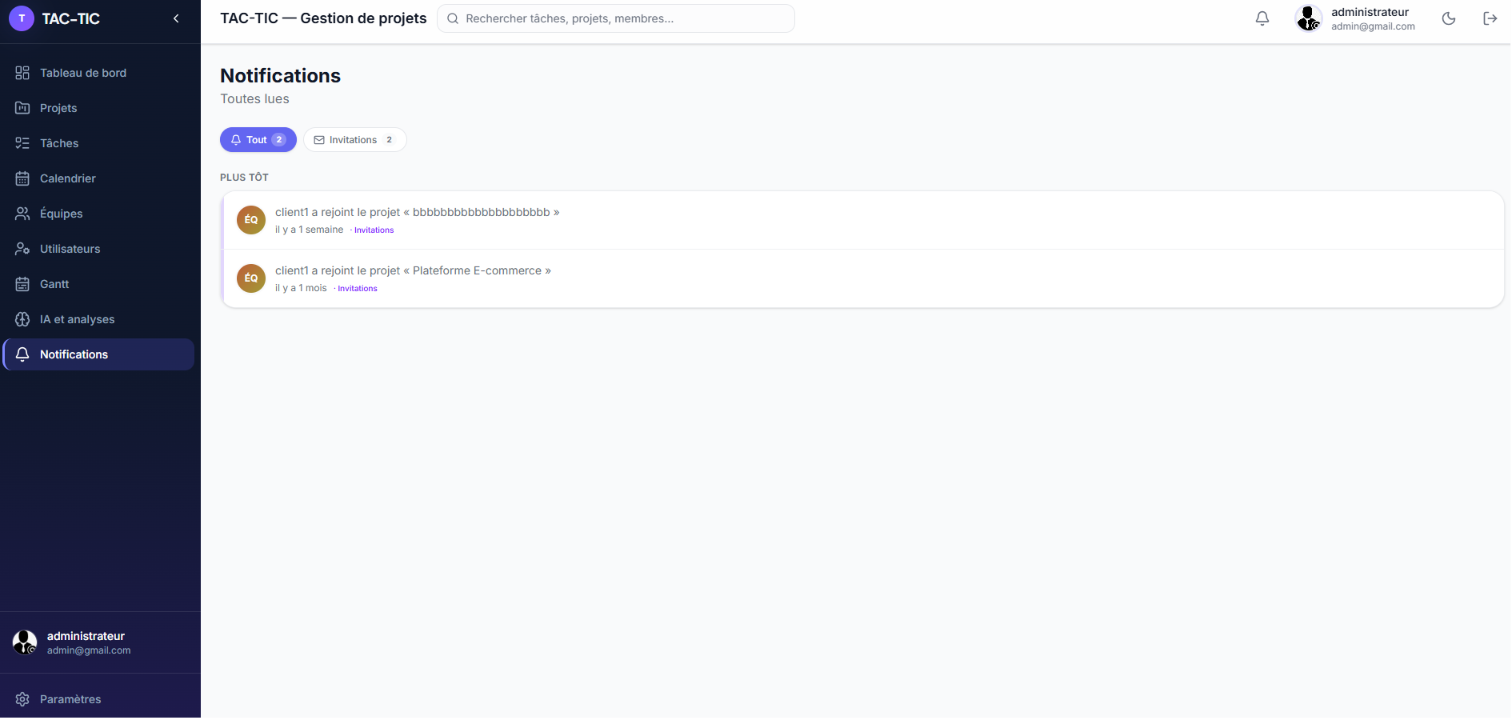
\includegraphics[width=0.80\textwidth]{figures/sprint4_21_notifications.png}%
  }{%
    \fbox{\parbox{0.80\textwidth}{\centering\vspace{2cm}
      \textbf{[IMAGE A INSÉRER]}\\[0.4em]
      \texttt{figures/sprint4\_21\_notifications.png}\\[0.3em]
      \textit{Centre de notifications : onglets Tout / Invitations / Retards, badge compteur}
    \vspace{2cm}}}%
  }
  \caption{Centre de notifications — Onglets et filtres}
  \label{fig:ui_notifications}
\end{figure}



% ============================================================
\subsection{Préférences utilisateur}

Chaque utilisateur dispose d'un panneau de préférences personnalisables accessible
depuis la page \textit{Paramètres → Notifications}. Les préférences sont persistées
en base de données dans la table \texttt{user\_preferences} et rechargées à chaque
session via l'endpoint \texttt{GET /api/auth/me}.

\begin{table}[H]
  \centering
  \caption{Préférences de notification disponibles}
  \label{tab:preferences_notif}
  \begin{tabularx}{\textwidth}{L{5cm}L{3cm}X}
    \toprule
    \thead{Préférence} & \thead{Type} & \thead{Description} \\
    \midrule
    \rowcolor{lightgray}
    Nouvelles invitations   & Bascule & Notifier à la réception d'une invitation projet \\
    Tâches assignées        & Bascule & Notifier lorsqu'une tâche est affectée \\
    \rowcolor{lightgray}
    Alertes de retard       & Bascule & Notifier lorsqu'une tâche dépasse sa date limite \\
    Mises à jour Kanban     & Bascule & Notifier lors d'un déplacement de carte \\
    \rowcolor{lightgray}
    Commentaires \& mentions & Bascule & Notifier lorsqu'un utilisateur vous mentionne \\
    Fréquence email digest  & Sélecteur & Jamais / Quotidien / Hebdomadaire \\
    \bottomrule
  \end{tabularx}
\end{table}

% ============================================================
\subsection{Synchronisation temps réel}

La synchronisation temps réel est assurée par \textbf{Laravel Reverb} (serveur
WebSocket natif Laravel) côté backend et la bibliothèque \textbf{Pusher JS} côté
React. Chaque utilisateur authentifié s'abonne automatiquement à son canal privé
\texttt{private-user.\{id\}} à l'ouverture de l'application.

\begin{table}[H]
  \centering
  \caption{Événements WebSocket diffusés par Laravel Reverb}
  \label{tab:websocket_events}
  \begin{tabularx}{\textwidth}{L{5cm}L{3cm}X}
    \toprule
    \thead{Événement} & \thead{Canal} & \thead{Déclencheur} \\
    \midrule
    \rowcolor{lightgray}
    \texttt{TaskMoved}      & Projet privé  & Déplacement d'une carte Kanban \\
    \texttt{TaskDelayed}    & Utilisateur   & Tâche dépassant sa date d'échéance \\
    \rowcolor{lightgray}
    \texttt{InvitationSent} & Utilisateur   & Invitation à rejoindre un projet \\
    \texttt{CommentAdded}   & Projet privé  & Nouveau commentaire avec mention \\
    \rowcolor{lightgray}
    \texttt{SprintStarted}  & Projet privé  & Démarrage d'un sprint \\
    \texttt{MLResult}       & Utilisateur   & Résultat d'une analyse IA disponible \\
    \bottomrule
  \end{tabularx}
\end{table}

La latence médiane mesurée entre la diffusion de l'événement et sa réception côté
React est inférieure à \textbf{20\,ms} en conditions normales (réseau local). En cas
de déconnexion, Pusher JS gère la reconnexion automatique avec backoff exponentiel.

% ============================================================
\subsection{Système de scoring intelligent}

TAC-TIC IntelliPM calcule pour chaque tâche un \textbf{score de risque} composite
(0--100), combinant plusieurs indicateurs :

\begin{table}[H]
  \centering
  \caption{Composantes du score de risque de tâche}
  \label{tab:score_risque}
  \begin{tabularx}{\textwidth}{L{5cm}C{2cm}X}
    \toprule
    \thead{Composante} & \thead{Poids} & \thead{Calcul} \\
    \midrule
    \rowcolor{lightgray}
    Retard prévu (CPM)     & 35\,\% & Float $\leq$ 0 → risque maximal \\
    Priorité               & 20\,\% & Critique = 100, Haute = 70, Moyenne = 40 \\
    \rowcolor{lightgray}
    Charge de l'assigné    & 20\,\% & (tâches ouvertes / capacité sprint) × 100 \\
    Prédiction ML retard   & 25\,\% & Probabilité retard × 100 (modèle GBM) \\
    \bottomrule
  \end{tabularx}
\end{table}

Le score est recalculé à chaque modification de tâche et à chaque exécution du
scheduler horaire. Il est affiché sur les cartes Kanban sous forme de pastille
colorée : vert ($<$ 30), orange (30--70), rouge ($>$ 70). Le tableau de bord projet
expose la distribution des scores de risque sous forme de jauge circulaire.

% ============================================================
\subsection{Statistiques et indicateurs KPI}

Les dashboards de TAC-TIC IntelliPM exposent des indicateurs de performance (KPI)
à trois niveaux de granularité :

\begin{table}[H]
  \centering
  \caption{Indicateurs KPI disponibles par niveau}
  \label{tab:kpi_niveaux}
  \begin{tabularx}{\textwidth}{L{3cm}L{5cm}X}
    \toprule
    \thead{Niveau} & \thead{KPI} & \thead{Description} \\
    \midrule
    \rowcolor{lightgray}
    Système (Admin) & Utilisateurs actifs / inactifs & Répartition par rôle et statut \\
    Système (Admin) & Projets par statut & En cours, terminés, archivés \\
    \rowcolor{lightgray}
    Projet          & Vélocité par sprint & Story points livrés vs. planifiés \\
    Projet          & Taux de complétion  & Tâches terminées / total × 100 \\
    \rowcolor{lightgray}
    Projet          & Indice de santé (0--100) & Agrégation de 5 sous-indicateurs \\
    Tâche           & Score de risque IA  & Composite CPM + ML + charge \\
    \rowcolor{lightgray}
    Tâche           & Temps passé vs. estimé & Comparaison heures réelles / estimées \\
    Membre          & Charge actuelle     & Nombre de tâches ouvertes et allocation \% \\
    \bottomrule
  \end{tabularx}
\end{table}

L'indice de santé projet est calculé à partir de cinq axes — délai, budget, qualité,
risque et moral d'équipe — visualisés sous forme de diagramme radar (Recharts). Un
score global $\geq$ 70 indique un projet sain ; entre 40 et 70, des vigilances sont
signalées ; en dessous de 40, une alerte est déclenchée.

% ============================================================
\section{Tests unitaires}

\begin{lstlisting}[style=phpstyle,caption={Tests unitaires — CPM et notifications},label={lst:tests_s4}]
it('identifies critical path tasks (float = 0)', function () {
    $project  = Project::factory()->withLinkedTasks(3)->create();
    $critical = app(CriticalPathService::class)->calculate($project);

    expect($critical)->not->toBeEmpty()
        ->and(collect($critical)->every(fn($t) => $t['float'] == 0))
        ->toBeTrue();
});

it('broadcasts delay notification', function () {
    Event::fake([TaskDelayed::class]);
    $task = Task::factory()->overdue()->create();

    app(NotificationService::class)->notifyDelay($task, $task->assignees);

    Event::assertDispatched(TaskDelayed::class);
});

it('marks notification as read', function () {
    $notif = Notification::factory()->unread()->create();
    $this->actingAs($notif->user)
         ->patchJson("/api/notifications/{$notif->id}/read")
         ->assertOk();
    expect($notif->fresh()->read_at)->not->toBeNull();
});
\end{lstlisting}

\begin{chapconclusion}
Le sprint~4 a livré 52 story points, le plus important du projet. Le Gantt avec
chemin critique a été le composant le plus complexe : la sérialisation topologique
du graphe de dépendances et le calcul CPM ont nécessité un soin particulier pour
gérer les cas limites (tâches sans dépendances, graphes déconnectés). Laravel Reverb
s'est montré très fiable avec une latence médiane inférieure à 20\,ms. Le scoring
intelligent et les KPI multi-niveaux offrent aux chefs de projet une visibilité
décisionnelle inédite.
\end{chapconclusion}
